%!TEX root = project.tex

\chapter*{About this project}
\paragraph{Abstract}
A brief description of what the willy is, in about two-hundred and fifty words.

\paragraph{Authors}
Explain here who the authors are.



\chapter{Introduction}
Throughout our college education we were embraced with the pressure of Projects, Assessments, with struggled deadlines and trying to keep track of a list of tasks to be completed. Good organisation is key to the success of a student and so we decided to create a system to assist students with their college organisation. We wanted to create a way for students to track events, have a look at their timetable and have keep track of assignments. We understood that it is important for students to keep track of their grades and their overall grade point average (GPA) for College. We decided to create a Student planner to help students keep track of the necessities in their college careers. 

Upon planning what we each wished to achieve from this project, we settle on gaining greater knowledge of the Java programming language. We then decided that this project should be a web application developed in J2EE which is Java 2 Platform, Enterprise Edition. J2EE provides the types of services that are necessary to build large scale, distributed, component based, multi-tier applications. Learning J2EE was new to us in the sense of using JSP, Servlets and incorporating other technologies to build this web application.[http://www.javaranch.com/journal/2002/10/J2EE.html]

\chapter{Context}
\begin{itemize}
\item Provide a context for your project.
\item Set out the objectives of the project
\item Briefly list each chapter / section and provide a 1-2 line description of what each section contains.
\item List the resource URL (GitHub address) for the project and provide a brief list of the main elements at the URL.
\end{itemize}

\section{Objectives}

\section{Project Links}
Links to this write up report, the main project repository and the URL to the Web Application which is currently being hosted on Heroku, can all be found below.

\paragraph{Links}
\begin{itemize}
\item https://github.com/Chrissweir/Final-Year-Project/blob/master/project.pdf
\item https://github.com/Chrissweir/Final-Year-Project
\item https://collegeplannerfyp.herokuapp.com/
\end{itemize}

\section{Chapters Review}
In this chapter we will briefly review the different areas of this paper. From the design and planning phase to the implementation phase.

\subsection{Methodology}
In this chapter we will cover the different development methodologies we used to develop this project, including weekly project meetings, collaboration tools used, application testing and weekly meetings with the project supervisors.

\subsection{Technology Review}
The different technologies used to design and implement the project from start to finish. The software development approaches to the tools used to create our application and the particular reasons for choosing the specified technologies.

\subsection{System Design}
This chapter will provide detailed information about the application system itself along with how it functions. This chapter also covers the architecture of the project, data models used, along with diagrams and screenshots.

\subsection{System Evaluation}
This chapter describes how we believe that our application is secure and robust through testing techniques that were used to test the application. We also discuss our initial objectives compared to our achieved goals, and highlight any of the limitation or opportunities in the technologies used.

\subsection{Conclusion}
This chapter summarises the context of our project and the conclusion from the overall design and development of the project, we will review the final version of the application and discuss different parts of the implementation that could have been developed differently.

\chapter{Methodology}

\section{Agile Development}

\section{Version Control}

\section{Testing}

About one to two pages.
Describe the way you went about your project:
\begin{itemize}
\item Agile / incremental and iterative approach to development. Planning, meetings.
\item What about validation and testing? Junit or some other framework.
\item If team based, did you use GitHub during the development process.
\item Selection criteria for algorithms, languages, platforms and technolo-gies.
\end{itemize}
Check out the nice graphs in Figure \ref{tikz:graphs}, and the nice diagram in Figure \ref{tikz:mydiagram}.

\begin{figure}
  \centering
  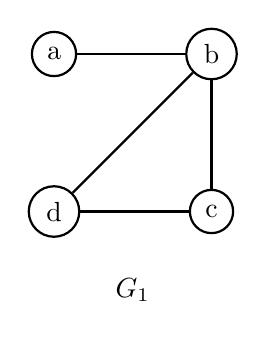
\begin{tikzpicture}
  \begin{scope}[every node/.style={circle,thick,draw}]
  \node (a) at (0,2) {a};
  \node (b) at (2,2) {b};
  \node (c) at (2,0) {c};
  \node (d) at (0,0) {d};
  \end{scope}
  \begin{scope}[every edge/.style={draw=black,thick}]
  \path (a) edge (b);
  \path (b) edge (c);
  \path (b) edge (d);
  \path (c) edge (d);
  \end{scope}
  \node () at (1,-1) {$G_1$};
  \end{tikzpicture}
  \hspace{1.5cm}
  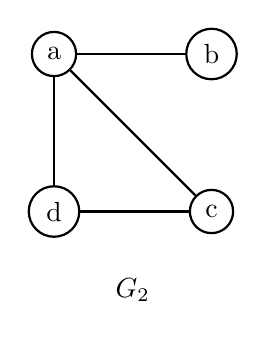
\begin{tikzpicture}
  \begin{scope}[every node/.style={circle,thick,draw}]
  \node (1) at (0,2) {a};
  \node (2) at (2,2) {b};
  \node (3) at (2,0) {c};
  \node (4) at (0,0) {d};
  \end{scope}
  \begin{scope}[every edge/.style={draw=black,thick}]
  \path (1) edge (2);
  \path (1) edge (3);
  \path (1) edge (4);
  \path (3) edge (4);
  \end{scope}
  \node () at (1,-1) {$G_2$};
  \end{tikzpicture}
  \caption{Nice pictures}
  \label{tikz:graphs}
\end{figure}


\begin{figure}
  \centering
  \begin{tikzpicture}[node distance=6cm]
  \node (a) [rect] {A Big Blue Block};
  \node (b) [oval, right of=a] {And His Oval Friend};
  \draw [line] (a) -- (b);
  \end{tikzpicture}
  \caption{Nice pictures}
  \label{tikz:graphs}
\end{figure}


\chapter{Technology Review}
About seven to ten pages.

In this section we're going to discuss the technology used
throughout the development of this project. This section will
briefly cover about the technologies and emphasize the reason for 
choosing these technologies. We used the Java EE(Java Enterprise Edition)
as our platform to develop this web application. We used MongoDB and MySQL
databases which are hosted on Heroku.

\section{Java EE}
The official documentation defines Java Platform, Enterprise Edition or 
Java EE as a widely used computing platform for developing, building and 
deploying Web-based enterprise applications online, which was formerly known as Java 2 Platform, Enterprise Edition 
or J2EE [http://www.oracle.com/technetwork/java/javaee/overview/index.html].
\par
The Java EE platform is built on top of the Java SE platform, which provides
an API for object-relational mapping and runtime environment for developing
large-scale, reliable, multitiered, scalable and secure web applications[http://docs.oracle.com/javaee/6/firstcup/doc/gkhoy.html].
At a client tier, Java EE supports Java applets or applications, as well as
HTML. It depends on Java Servlet Pages and servlet code to create and process
HTML or other formatted data for the client[http://www.webopedia.com/TERM/J/J2EE.html].
\subsection{JSP}
JavaServer Pages is a technology that provides web developers with a framework to create dynamically generated web pages using HTML, XML and java code which is secure, fast and independent of server platform [http://www.oracle.com/technetwork/articles/javase/jsp-135132.html]. JSP
is similar to PHP and ASP but uses the java programming laguage.
\par
JavaServer Pages have dynamic scripting capabilities that work in conjunction with HTML code, which seperates the page logic from the static elements (the actual design and display of the page), to help make the HTML more functional
[http://www.webopedia.com/TERM/J/JSP.html]. In order to deploy and run JavaServer Pages, a compatible web server with a servlet container, such as Apache Tomcat is required.\\
\\
\textbf{Example:}
\begin{minted}{jsp}
<html>
    <body>
        <!-- JSP file format -->
        <%
            out.println ("Hello World");
        %>
    </body>
</html>
\end{minted}
\textbf{Result:}\\
Hello World

\subsection{Servlets}

\subsection{XML}
XML stands for Extensible Markup Language. XML was designed to store and transport data and was designed to be both human- and machine-readable. XML data is known as self-describing or self-defining, meaning that the structure of the data is embedded with the data, thus when the data arrives there is no need to pre-build the structure to store the data; it is dynamically understood within the XML[http://searchmicroservices.techtarget.com/definition/XML-Extensible-Markup-Language].
\begin{minted}{xml}
<this>
  <looks lookswhat="good">
    Good
  </looks>
</this>
\end{minted}

\subsection{Tomcat}
Apache Tomcat, often referred to as Tomcat, is an open source Java Servlet Container that implements several Java EE specifications including Java Servlet, JavaServer Pages, Java Expression Language and Java WebSocket technologies[http://tomcat.apache.org/]. Tomcats core component is the servlet container Catalina, when the Tomcat server is being started it is actually Catalina being started. Catalina implements Sun Microsystems' specifications for servlet and JavaServer Pages (JSP).

\section{Heroku}
Heroku is a container-based cloud Platform as a Service. Heroku is used by developers to deploy, manage and scale modern apps. Heroku’s platform is elegant, flexible and manageable which offers developers a straightforward path when getting their apps to market. This was an obvious benefit to us when choosing what platform to integrate into our project. Heroku is fully managed which gives developers the freedom to focus on their core product without having to maintain servers, hardware or infrastructure. Heroku provides services, tools, workflows and polyglot support all of which enhances the developer’s productivity [https://www.heroku.com/about].

\subsection{MongoDB}
MongoDB is a free, open source cross-platform database program. It is document-oriented which means it is designed for storing, retrieving and managing document-orientated information. This is also known as semi structured data. MongoDB is a NoSQL database program and uses JSON-like documents with schemas. MongoDB is a distributed database and is designed for ease of development and scaling and also possesses satisfying scalability and flexibility. The document model maps to the objects in your application code which makes data easy to work with. Ad hoc queries, indexing, and real time aggregation provide powerful ways to access and analyse your data[https://www.mongodb.com/what-is-mongodb]. \par Having previous knowledge of MongoDB stood to us during the development of our project and that along with it being document based which made it more suitable over using a file server helped us in making a decision when choosing a database to use for our project. MongoDB has a range of features that were beneficial to us throughout the duration of this project. For file storage, large objects or files are easily stored within MongoDB. MongoDB supports an easy to use protocol for storing large files and files metadata. Incredible performance is a major goal for MongoDB and has therefore shaped much of its design[MongoDb book].

\subsection{MySQL}
MySQL is an open source SQL database management system which is developed, distributed and supported by Oracle Corporation. MySQL is a relational database that stores data in separate tables rather than storing it all together in one big clump of data. These database structures are organized into physical files optimized for speed. MySQL provides a flexible programming environment with its tables, views, rows and columns. Relationships such as one-to-one, one-to-many, unique, required and optional can be created so as that your application never sees inconsistent, missing or out-of-date data. Depending on what way you would like to populate your MySQL database, there are various different way in which you can enter information. You may enter it directly such as generating reports, use a language specific API that hides the SQL syntax or embed SQL statements into your code written in another language. MySQL is a client/server system which consists of a multi-threaded SQL server. It supports different back ends, several different client programs and libraries and a wide range of application programming interfaces(APIs). MySQL also scales up to clusters of machines networked together.\par The MySQL Database server a rich and useful set of functions and is fast, reliable, scalable and relatively easy to use which influenced our decision when choosing what technologies we would like to work with on our project. We had used MySQL on previous which benefitted us during the development of our College Planner website. MySQL’s connectivity, speed, and security makes it very suitable when accessing databases on the internet.


\section{Bootstrap}
Bootstrap is a free, open source front-end web framework for designing web applications for enhanced user experience and design. It contains HTML and CSS based design templates for forms, buttons, navigation, and other interface components. Bootstrap is front-end development only and has a great range of features that enhanced our project design [https://blog.getbootstrap.com/]. \par Bootstrap is great for speed of development, this is because bootstrap lets you utilize ready made code to program website design for your own benefit. Bootstrap also has good responsiveness and consistency as bootstrap is continuously updated and made sure the framework is bug-free. In addition, results are uniform across platforms so output remains the same whether you’re using Firefox, Chrome or Internet Explorer. [https://bootstrapbay.com/blog/reasons-to-use-bootstrap/].

\section{JQuery}
JQuery is a fast and concise JavaScript Library with the purpose of making it much easier to use JavaScript on your website. It's a lightweight, "write less, do more", which means jQuery takes a lot of common tasks that requires many lines of JavaScript code to accomplish, and wraps them into methods that you can call with a single line of code [https://www.tutorialspoint.com/jquery/jquery-overview.htm]. Jquery is a very lightweight library and is Cross Browser Support which is what we need for our application.

\begin{itemize}
\item Describe each of the technologies you used at a conceptual level. Standards, Database Model (e.g. MongoDB, CouchDB), XMl, WSDL, JSON, JAXP.
\item Use references (IEEE format, e.g. [1]), Books, Papers, URLs (timestamp) – sources should be authoritative. 
\end{itemize}



\chapter{System Design}

\section{System Backend}

\subsection{Databases}

\subsection{Servlets}

\section{Front End (JSP)}

\subsection{Login/Register}

\subsection{Account Recovery}

\subsection{Profile}

\subsection{Calendar}

\subsection{Timetable}

\subsection{To do List}

\subsection{Modules}

\subsection{Assignments}

\subsection{Scripts and Styling}

\section{UML}

As many pages as needed.
\begin{itemize}
\item Architecture, UML etc. An overview of the different components of the system. Diagrams etc… Screen shots etc.
\end{itemize}

\begin{table}[h]
  \centering
  \begin{tabular}{x{2cm}p{3cm}}
    \toprule \\
    Column 1 & Column 2 \\
    \midrule \\
    Rows 2.1 & Row 2.2 \\
    \bottomrule
  \end{tabular}
  \caption{A table.}
  \label{table:mytable}
\end{table}

\chapter{System Evaluation}

\section{Testing}

\subsection{Selenium}

\subsection{JUnit}

\section{Outcomes VS. Objectives}

\section{Limitations}

As many pages as needed.
\begin{itemize}
\item Prove that your software is robust. How? Testing etc. 
\item Use performance benchmarks (space and time) if algorithmic.
\item Measure the outcomes / outputs of your system / software against the objectives from the Introduction.
\item Highlight any limitations or opportuni-ties in your approach or technologies used.
\end{itemize}

\chapter{Conclusion}
About three pages.

\begin{itemize}
\item Briefly summarise your context and ob-jectives (a few lines).
\item Highlight your findings from the evalua-tion section / chapter and any opportunities identified.
\end{itemize}